% Options for packages loaded elsewhere
\PassOptionsToPackage{unicode}{hyperref}
\PassOptionsToPackage{hyphens}{url}
%
\documentclass[
]{article}
\usepackage{amsmath,amssymb}
\usepackage{lmodern}
\usepackage{ifxetex,ifluatex}
\ifnum 0\ifxetex 1\fi\ifluatex 1\fi=0 % if pdftex
  \usepackage[T1]{fontenc}
  \usepackage[utf8]{inputenc}
  \usepackage{textcomp} % provide euro and other symbols
\else % if luatex or xetex
  \usepackage{unicode-math}
  \defaultfontfeatures{Scale=MatchLowercase}
  \defaultfontfeatures[\rmfamily]{Ligatures=TeX,Scale=1}
\fi
% Use upquote if available, for straight quotes in verbatim environments
\IfFileExists{upquote.sty}{\usepackage{upquote}}{}
\IfFileExists{microtype.sty}{% use microtype if available
  \usepackage[]{microtype}
  \UseMicrotypeSet[protrusion]{basicmath} % disable protrusion for tt fonts
}{}
\makeatletter
\@ifundefined{KOMAClassName}{% if non-KOMA class
  \IfFileExists{parskip.sty}{%
    \usepackage{parskip}
  }{% else
    \setlength{\parindent}{0pt}
    \setlength{\parskip}{6pt plus 2pt minus 1pt}}
}{% if KOMA class
  \KOMAoptions{parskip=half}}
\makeatother
\usepackage{xcolor}
\IfFileExists{xurl.sty}{\usepackage{xurl}}{} % add URL line breaks if available
\IfFileExists{bookmark.sty}{\usepackage{bookmark}}{\usepackage{hyperref}}
\hypersetup{
  pdftitle={Christmas carols: multi-lingual, with chords, analyzed using Data Science},
  hidelinks,
  pdfcreator={LaTeX via pandoc}}
\urlstyle{same} % disable monospaced font for URLs
\usepackage[margin=1in]{geometry}
\usepackage{graphicx}
\makeatletter
\def\maxwidth{\ifdim\Gin@nat@width>\linewidth\linewidth\else\Gin@nat@width\fi}
\def\maxheight{\ifdim\Gin@nat@height>\textheight\textheight\else\Gin@nat@height\fi}
\makeatother
% Scale images if necessary, so that they will not overflow the page
% margins by default, and it is still possible to overwrite the defaults
% using explicit options in \includegraphics[width, height, ...]{}
\setkeys{Gin}{width=\maxwidth,height=\maxheight,keepaspectratio}
% Set default figure placement to htbp
\makeatletter
\def\fps@figure{htbp}
\makeatother
\setlength{\emergencystretch}{3em} % prevent overfull lines
\providecommand{\tightlist}{%
  \setlength{\itemsep}{0pt}\setlength{\parskip}{0pt}}
\setcounter{secnumdepth}{-\maxdimen} % remove section numbering
\ifluatex
  \usepackage{selnolig}  % disable illegal ligatures
\fi

\title{Christmas carols: multi-lingual, with chords, analyzed using Data
Science}
\author{}
\date{\vspace{-2.5em}\url{https://rpubs.com/ivim/noel}
({[}\url{https://gorodnichy.github.io}{]}/noel(\url{https://gorodnichy.github.io\%5D/noel}))}

\begin{document}
\maketitle

{
\setcounter{tocdepth}{4}
\tableofcontents
}
\hypertarget{merry-christmas-tout-le-monde}{%
\subsection*{Merry Christmas, tout le monde
!}\label{merry-christmas-tout-le-monde}}
\addcontentsline{toc}{subsection}{Merry Christmas, tout le monde !}

Voici sont les meilleures chansons de Noël et d'hiver for holiday season
- in English, en français, and other languages - with chords and
analyzed using data science techniques. The image below shows the
graphical representation of the result - the most frequent words used to
describe the holiday spirit in each language.

\begin{figure}

{\centering 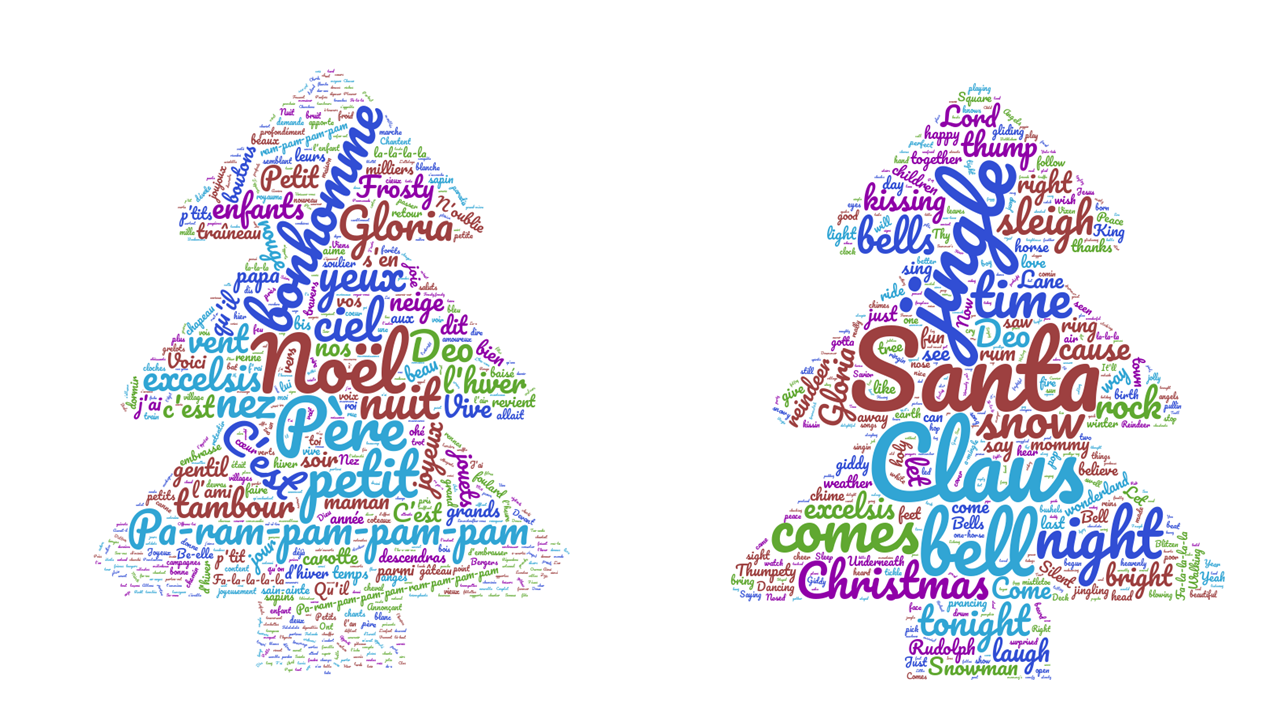
\includegraphics[width=0.99\linewidth,height=0.2\textheight]{noel-songs-wordcloud} 

}

\caption{Figure 1: Data representation of Christmas songs in this booklet: 
English vs. French versions of the same songs }\label{fig:unnamed-chunk-2}
\end{figure}

Songs are organized by the language origin: with those having multiple
language versions appearing first, followed by New Year songs and other
winter songs. Less known songs are accompanied by links to listen them
on SoundCloud.

A pdf version of this document for printing or reading with e-reader is
available \href{https://ivi-m.github.io/noel/noel.pdf}{here}. Enjoy!

\hypertarget{other-resources}{%
\paragraph*{Other resources}\label{other-resources}}
\addcontentsline{toc}{paragraph}{Other resources}

\href{https://en.wikipedia.org/wiki/List_of_Christmas_carols}{List of
Christmas Carols in wikipedia}

\hypertarget{chord-notation}{%
\paragraph*{Chord notation}\label{chord-notation}}
\addcontentsline{toc}{paragraph}{Chord notation}

``\textbar{}'' or blank indicate the end of measure,
``\textbar\textbar{}'' - end of line, and indent - new melody part or
refrain. H is Si/Ti major chord (B in standard notation) and B is Si/Ti
flat major chord (Bb in standard notation). The rest follows the
\href{https://en.wikipedia.org/wiki/Chord_letters}{standard chord
notation}.

Contributions and corrections welcome! Email them to
\texttt{dg\ @\ ivim.ca} or fork the
\href{https://github.com/gorodnichy/noel}{source github repo}

\hypertarget{credits}{%
\subsubsection*{Credits}\label{credits}}
\addcontentsline{toc}{subsubsection}{Credits}

This book is generated automatically from the
\href{https://rmarkdown.rstudio.com/}{R Markdown} script in
\href{https://rstudio.cloud}{RStudio}. The source is at
\href{https://github.com/IVI-M/noel}{GitHub}.\\
The lyrics is analyzed using R. The chords and data analysis are
provided by \href{http://www.gorodnichy.ca}{Dmitry Gorodnichy}.

\begin{center}\rule{0.5\linewidth}{0.5pt}\end{center}

\hypertarget{o-tannenbaum---mon-beau-sapin---christmas-tree}{%
\section{O Tannenbaum - Mon beau sapin - Christmas
Tree}\label{o-tannenbaum---mon-beau-sapin---christmas-tree}}

\hypertarget{section}{%
\subsection*{}\label{section}}
\addcontentsline{toc}{subsection}{}

\begin{verbatim}
C C  || G C
    G G7 ||  G7 C || C C || G C || 
\end{verbatim}

\hypertarget{mon-beau-sapin}{%
\subsubsection*{Mon beau sapin}\label{mon-beau-sapin}}
\addcontentsline{toc}{subsubsection}{Mon beau sapin}

\begin{verbatim}
Mon beau sapin, roi des forêts 
Que j'aime ta verdure! (x2)

  Quand, par l'hiver, bois et guérets 
  Sont dépouillés de leurs attraits 
  Mon beau sapin, roi des forêts 
  Tu gardes ta parure.
\end{verbatim}

\hypertarget{christmas-tree}{%
\subsubsection*{Christmas Tree}\label{christmas-tree}}
\addcontentsline{toc}{subsubsection}{Christmas Tree}

\begin{verbatim}
O Christmas tree, O Christmas tree
Your leaves are so unchanging (x2)

  Not only green when Summer’s here
  But also when it’s cold and drear
  O Christmas tree, O Christmas tree
  Your leaves are so unchanging
\end{verbatim}

\hypertarget{o-tannenbaum}{%
\subsubsection*{O Tannenbaum}\label{o-tannenbaum}}
\addcontentsline{toc}{subsubsection}{O Tannenbaum}

\begin{verbatim}
 O Tannenbaum, o Tannenbaum,
 Dein Kleid will mich was lehren: (x2)
 
   Die Hoffnung und Beständigkeit
   Gibt Mut und Kraft zu jeder Zeit!
   O Tannenbaum, o Tannenbaum,
   Dein Kleid will mich was lehren!
\end{verbatim}

\hypertarget{stille-nacht---silent-night---douce-nuit-sainte-nuit---ux442ux438ux445ux430-ux43dux456ux447}{%
\section{Stille Nacht - Silent night - Douce Nuit Sainte Nuit - Тиха
ніч}\label{stille-nacht---silent-night---douce-nuit-sainte-nuit---ux442ux438ux445ux430-ux43dux456ux447}}

\hypertarget{section-1}{%
\subsection*{}\label{section-1}}
\addcontentsline{toc}{subsection}{}

\begin{verbatim}
C C G C
F C F C
Dm G Am Am7/G
C G C C
\end{verbatim}

\hypertarget{stille-nacht}{%
\subsubsection*{Stille Nacht}\label{stille-nacht}}
\addcontentsline{toc}{subsubsection}{Stille Nacht}

\begin{verbatim}
Stille Nacht, heilige Nacht,
Alles schläft; einsam wacht
Nur das traute hochheilige Paar.
Holder Knabe im lockigen Haar,
Schlaf in himmlischer Ruh!
Schlaf in himmlischer Ruh!

Stille Nacht, heilige Nacht,
Hirten erst kundgemacht
Durch der Engel Halleluja,
Tönt es laut von fern und nah:
Christ, der Retter ist da!
Christ, der Retter ist da!

Stille Nacht, heilige Nacht,
Gottes Sohn, o wie lacht
Lieb' aus deinem göttlichen Mund,
Da uns schlägt die rettende Stund'.
Christ, in deiner Geburt!
Christ, in deiner Geburt
\end{verbatim}

\href{https://omniglot.com/songs/multilingual/silentnight/index.php}{In
other languages}

\hypertarget{douce-nuit-sainte-nuit}{%
\subsubsection*{Douce Nuit Sainte Nuit}\label{douce-nuit-sainte-nuit}}
\addcontentsline{toc}{subsubsection}{Douce Nuit Sainte Nuit}

\begin{verbatim}
Be-elle nuit, sain-ainte nuit!
Tout s'endort, plus de bruit.
Veille seu-eul, le  couple sacré
Doux enfan-ant aux  fin-ins cheveux
Clos tes yeux et repo--s e.
Sou-ous cesyeux vigilants.

Be-elle nuit, sain-ainte nuit! 
Dans les champs, les bergers, 
Par les an-anges a-avertis, 
Font partou-out retentir leur voix: 
Le sauveur vient de naî-aî-tre 
Le-e sauveu-eur est là! 

Be-elle nuit, sain-ainte nuit! 
Mon Jésus bien aimé, 
Quel souri-ire dan-ans tes yeux, 
Tan-andis que pour l'ho-o-om-me 
So-onne l'heure sainte, 
L'heu-eure du-u salut! 
\end{verbatim}

\hypertarget{silent-night}{%
\subsubsection*{Silent night}\label{silent-night}}
\addcontentsline{toc}{subsubsection}{Silent night}

\begin{verbatim}
Silent night, holy night! 
All is calm, all is bright. 
Round yon Virgin, Mother and Child. 
Holy infant so tender and mild, 
Sleep in heavenly peace, 
Sleep in heavenly peace. 

Silent night, holy night! 
Shepherds quake at the sight. 
Glories stream from heaven afar 
Heavenly hosts sing Alleluia, 
Christ the Savior is born! 
Christ the Savior is born. 

Silent night, holy night! 
Son of God love's pure light. 
Radiant beams from Thy holy face 
With dawn of redeeming grace, 
Jesus Lord, at Thy birth. 
Jesus Lord, at Thy birth.
\end{verbatim}

\hypertarget{ukrainian}{%
\subsubsection*{Ukrainian}\label{ukrainian}}
\addcontentsline{toc}{subsubsection}{Ukrainian}

\begin{verbatim}
Тиха ніч
Тиха ніч, свята ніч!
Ясність б'є від зірниць.
Дитинонька Пресвята,
Така ясна, мов зоря,
Спочиває в тихім сні.

Тиха ніч, свята ніч!
Ой, зітри сльози з віч,
Бо Син Божий йде до нас,
Цілий світ любов'ю спас,
Вітай нам, святе Дитя!

Свята ніч настає,
Ясний блиск з неба б'є,
В людськім тілі Божий Син
Прийшо нині в Вифлеєм
Щоб спасти цілий світ.

Тиха ніч, свята ніч!
Зірка сяє ясна,
Потішає серця,
Величає Христа.
Дитя святе, як зоря,
Нам світи, зоря ясна!
\end{verbatim}

\hypertarget{deck-the-halls---falalalala}{%
\section{Deck the Halls -
Falalalala}\label{deck-the-halls---falalalala}}

\hypertarget{section-2}{%
\subsection*{}\label{section-2}}
\addcontentsline{toc}{subsection}{}

\begin{verbatim}
C  G  C  ||  C  G  C 
      G C F C  ||   C  G  C
\end{verbatim}

\hypertarget{english}{%
\subsubsection*{English}\label{english}}
\addcontentsline{toc}{subsubsection}{English}

\begin{verbatim}
Deck the Halls

Deck the halls with boughs of holly
Fa-la-la-la-la, la-la-la-la
'Tis the season to be jolly
Fa-la-la-la-la, la-la-la-la

  Don we now our gay apparel
  Fa-la-la, la-la-la, la-la-la.
  Troll the ancient Yule-tide carol
  Fa-la-la-la-la, la-la-la-la.
\end{verbatim}

\hypertarget{franuxe7ais}{%
\subsubsection*{Français}\label{franuxe7ais}}
\addcontentsline{toc}{subsubsection}{Français}

\begin{verbatim}
Falalalala

Dans les villes et les villages 
Fa-la-la-la-la, la-la-la-la
Répandons notre message 
Fa-la-la-la-la, la-la-la-la

  Proclamons la joie profonde 
  Fa-la-la, la-la-la, la-la-la
  Que Dieu a donné au monde 
  Fa-la-la-la-la, la-la-la-la

Que l'on chante qu'on s'apprête
Fa la la la la la la la la
Sonnez pipeaux et trompettes
Fa la la la la la la la la

  Car c'est la joie qu'on apporte
  Fa la la la la la la la la
  Ouvrez donc grandes vos portes
  Fa la la la la la la la la
\end{verbatim}

\hypertarget{jingle-bells---vive-le-vent---ux434ux437ux435ux43dux44c-ux434ux437ux435ux43bux435ux43dux44c---ux431ux443ux431ux435ux43dux446ux44b}{%
\section{Jingle Bells - Vive le vent - Дзень-дзелень -
Бубенцы}\label{jingle-bells---vive-le-vent---ux434ux437ux435ux43dux44c-ux434ux437ux435ux43bux435ux43dux44c---ux431ux443ux431ux435ux43dux446ux44b}}

\hypertarget{section-3}{%
\subsection*{}\label{section-3}}
\addcontentsline{toc}{subsection}{}

\begin{verbatim}
C  || Dm || G || C
       C C || C C || F C || D G
\end{verbatim}

\hypertarget{english-1}{%
\subsubsection*{English}\label{english-1}}
\addcontentsline{toc}{subsubsection}{English}

\begin{verbatim}
Jingle Bells

Dashing through the snow
In a one horse open sleigh
Over fields we go
Laughing all the way
Bells on bob tails ring
Making spirits bright
What fun it is to laugh and sing
A sleighing song tonight

  Oh, jingle bells, jingle bells
  Jingle all the way
  Oh, what fun it is to ride
  In a one horse open sleigh 
  (x2)
\end{verbatim}

\href{https://omniglot.com/songs/multilingual/jinglebells/german.php}{In
other languages}

\hypertarget{franuxe7ais-1}{%
\subsubsection*{Français}\label{franuxe7ais-1}}
\addcontentsline{toc}{subsubsection}{Français}

\begin{verbatim}
Vive le vent

Sur le long chemin 
Tout blanc de neige blanche 
Un vieux monsieur s'avance 
Avec sa canne dans la main 
Et tout là-haut le vent 
Qui siffle dans les branches 
Lui souffle la romance 
Qu'il chantait petit enfant:

  Vive le vent, vive le vent 
  Vive le vent d'hiver 
  Qui s'en va sifflant, soufflant 
  Dans les grands sapins verts 
  OH! Vive le temps, vive le temps 
  Vive le temps d'hiver 
  Boule de neige et jour de l'an 
  Et bonne année grand-mère ... 

    Joyeux joyeux Noël 
    aux mille bougies 
    qu'enchantent vers le ciel   
    les cloches de la nuit.
    
  Vive le vent, vive le vent,
  Vive le vent d'hiver 
  qui rapporte aux vieux enfants
  un souvenir d'hier.
\end{verbatim}

\hypertarget{ukrainian-1}{%
\subsubsection*{Ukrainian}\label{ukrainian-1}}
\addcontentsline{toc}{subsubsection}{Ukrainian}

\begin{verbatim}
Дзень-дзелень 

Срібно-білий сніг
Вистеле поріг.
Кличе у світи
Серпантин доріг.
За вікнами імла
І в пошуках тепла
По вулиці засніженій
Іде-бреде зима.
 
  Цілий день дзень-дзелень
  Дзвоники дзвенять.
  Ялинкові ліхтарі
  Казково мерехтять. Хей!
  Цілий день дзень-дзелень
  Ділі-дон-дін-дін.
  Зірка сяє і лунає
  Цей різдвяний дзвін.
 
Миколай іде.
Хор янголів веде.
Вітер-сніговій
У димар гуде.
Ми зичимо усім
Дорослим і малим
У цю чарівну світлу ніч
Знайти свій теплий дім.
 
Refrain
 
Подарунків міх:
Ласощі та сміх.
Щастя і добра
Вистачить на всіх.
Дивися, на вікні
Дерева крижані –
Це Новий Рік летить до нас
На білому коні.
 
Refrain.
\end{verbatim}

\hypertarget{russian}{%
\subsubsection*{Russian}\label{russian}}
\addcontentsline{toc}{subsubsection}{Russian}

\begin{verbatim}
Бубенцы

Бьёт в лицо нам снег,
Ветерок свистит,
Но задорный смех
Душу веселит.
С песней по полям
Радостно лететь,
Колокольчик нам
Помогает петь.

 Бубенцы, бубенцы
 Весело звенят,
 Нам с тобой так хорошо
 Кататься на санях!
 Динь-дeнь-дoн, динь-дeнь-дoн,
 Бубенцы звенят
 Ах, весело нам всем
 Кататься на санях!
 
Ах, какая прыть,
Словно ветер, мчимся мы,
Вовек нам не забыть
Красавицы-зимы!
Куда ни кинешь взгляд —
Сугробы да холмы,
Ну есть ли лучше время
Красавицы-зимы?
\end{verbatim}

\hypertarget{we-wish-you-a-merry-christmas---on-se-dit-joyeux-nouxebl}{%
\section{We wish you a Merry Christmas - On se dit Joyeux
Noël}\label{we-wish-you-a-merry-christmas---on-se-dit-joyeux-nouxebl}}

\hypertarget{section-4}{%
\subsection*{}\label{section-4}}
\addcontentsline{toc}{subsection}{}

\begin{verbatim}
C Dm ||  Dm G ||  E Am  ||  Dm G C 
       C G || G C || C Dm || G C|| 
\end{verbatim}

\hypertarget{english-2}{%
\subsubsection*{English}\label{english-2}}
\addcontentsline{toc}{subsubsection}{English}

\begin{verbatim}
We wish you a Merry Christmas (x3)
And a Happy New Year

  Good tidings we bring
  To you and your kin
  We wish you a Merry Christmas
  And a Happy New Year

Now bring us some figgy pudding (x3)
And a cup of good cheer
\end{verbatim}

\hypertarget{on-se-dit-joyeux-nouxebl}{%
\subsubsection*{On se dit Joyeux Noël}\label{on-se-dit-joyeux-nouxebl}}
\addcontentsline{toc}{subsubsection}{On se dit Joyeux Noël}

\begin{verbatim}
Je te dis joyeux Noël 
Tu me dis joyeux Noël 
On se dit joyeux Noël 
Et aussi bonne année

  A tout' la famille
  On dit joyeux Noël
  Et nos voeux pour que brille
  La nouvelle année

J'apporte un petit gâteau 
Tu apportes un petit gâteau 
On apporte un petit gâteau 
Petits gâteaux sucrés

Je donne un petit baisé
Tu donnes un petit baisé
On donne un petit baisé
Petits baisers mouillés

Et je ne partirai pas 
Et tu ne partiras pas 
Et on ne partira pas 
Avant davoir chanté
\end{verbatim}

\hypertarget{let-it-snow---cest-lhiver}{%
\section{Let it snow - C'est l'hiver}\label{let-it-snow---cest-lhiver}}

\hypertarget{section-5}{%
\subsection*{}\label{section-5}}
\addcontentsline{toc}{subsection}{}

\begin{verbatim}
(G) C C  ||  G G ||  Dm Dm || G C ||
      G G ||  D G ||  G G ||  D7 G
\end{verbatim}

\hypertarget{cest-lhiver}{%
\subsubsection*{C'est l'hiver}\label{cest-lhiver}}
\addcontentsline{toc}{subsubsection}{C'est l'hiver}

\begin{verbatim}
Nous filons sur la neige blanche
En ce beau jour de dimanche
À travers les sapins verts
C'est l'hiver, c'est l'hiver, c'est l'hiver

Les enfants de notre village
Chantent la joie de leur âge
Et les grands murmures de se taire
C'est l'hiver, c'est l'hiver, c'est l'hiver

  Le bon Dieu dans son paradis
  Doit aussi chanter avec nous
  Car la nature est si jolie
  Le bleu de son ciel est si doux
\end{verbatim}

\hypertarget{let-it-snow}{%
\subsubsection*{Let it snow}\label{let-it-snow}}
\addcontentsline{toc}{subsubsection}{Let it snow}

\begin{verbatim}
Oh, the weather outside is frightful
But the fire is so delightful
And since we've no place to go
Let it snow, let it snow, let it snow

Man it doesn't show signs of stoppin'
And I brought some corn for poppin'
The lights are turned way down low
Let it snow, let it snow, let it snow

  When we finally kiss goodnight
  How I’ll hate going out in the storm
  And if you only hold me tight,
  All the way home I’ll be warm

The fire is slowly dying
And my dear we're still goodbye-ing
As long as you love me so
Let it snow, let it snow, let it snow
\end{verbatim}

\hypertarget{ukrainian-2}{%
\subsubsection*{Ukrainian}\label{ukrainian-2}}
\addcontentsline{toc}{subsubsection}{Ukrainian}

\begin{verbatim}
Подарунки для нас тримає,
До шкарпеток вночі ховає,
Ти ім'я його заспівай:
Миколай! Миколай! Миколай!
Заспівають сніжинки білі
В порцеляновій заметілі,
Стане на наш поріг
Новий Рік! Новий Рік!
Як у небі зоря зійде,
Розпочнуться дива ураз,
Світла радість у дім іде -
Казка настане для нас!
Сяє вулиця ліхтарями,
Усміхнеться дитя до мами,
Нумо разом свято назвемо:
Це Різдво! Це Різдво!
Це Різдво!

Як у небі зоря зійде,
Розпочнуться дива ураз,
Світла радість у дім іде -
Казка настане для нас!
Подарунки для нас тримає,
До шкарпеток вночі ховає,
Ти ім'я його заспівай:
Миколай! Миколай! Миколай!
Пригорни, коли хтось сумує,
Новий Рік Ангела дарує,
Хай любов'ю світ обійма
Ця зима! Ця зима! Ця зима!
Ця зима! Ця зима! Ця зима!
Хай любов'ю нас всіх
Вона з вами обійма!
З Новим Роком!
\end{verbatim}

\hypertarget{russian-1}{%
\subsubsection*{Russian}\label{russian-1}}
\addcontentsline{toc}{subsubsection}{Russian}

\begin{verbatim}
Снова с неба летят снежинки
К нам на шляпы, на ботинки,
И сердце уже поет:
"Новый Год, Новый Год, Новый Год!"

Прохожий несет подарки,
Шуршит бумагой яркой,
И в гости спешит народ,
К нам идет Новый Год, Новый Год!

Если в дверь позвонят - открой,
Этой ночью возможно все!
Там стоит Дед Мороз седой,
Сказка стучится в окно!

И твой поцелуй украдкой
Со вкусом шоколадки - 
Сюрпризы нам раздает
Новый Год, Новый Год, Новый Год!

К нам идет Новый Год!

Если в дверь позвонят - открой,
Этой ночью возможно все!
Ровно в полночь глаза закрой,
Сказка стучится в окно!

Снова с неба летят снежинки
К нам на шляпы, на ботинки,
И сердце уже поет:
"Новый Год, Новый Год, Новый Год!"

Новый Год, Новый Год, Новый Год!
К нам идет Новый Год!
\end{verbatim}

\hypertarget{in-excelsis-deo---les-anges-dans-nos-campagnes}{%
\section{In Excelsis Deo - Les anges dans nos
campagnes}\label{in-excelsis-deo---les-anges-dans-nos-campagnes}}

\hypertarget{section-6}{%
\subsection*{}\label{section-6}}
\addcontentsline{toc}{subsection}{}

\begin{verbatim}
C || C || C || C C G C 
   C A7 Dm G C Dm G G7
     C G C F C G 
\end{verbatim}

\hypertarget{les-anges-dans-nos-campagnes}{%
\subsubsection*{Les anges dans nos
campagnes}\label{les-anges-dans-nos-campagnes}}
\addcontentsline{toc}{subsubsection}{Les anges dans nos campagnes}

\begin{verbatim}
Les anges dans nos campagnes 
Ont entonné l'hymne des cieux, 
Et l'écho de nos montagnes 
Redit ce chant mélodieux 

  Glo-o-o-o-o-o-o-o-o-o-o-o-oria 
    in excelsis Deo 
  x2

Bergers, pour qui cette fête ? 
Quel est l'objet de tous ces chants ? 
Quel vainqueur, quelle conquête 
Mérite ces cris triomphants : 

  Refrain

Ils annoncent la naissance 
Du libérateur d'Israël 
Et pleins de reconnaissance 
Chantent en ce jour solennel : 

  Refrain
  
Cherchons tous l'heureux village 
Qui l'a vu naître sous ses toits 
Offrons-lui le tendre hommage 
Et de nos cœurs et de nos voix : 

  Refrain

Bergers, quittez vos retraites, 
Unissez-vous à leurs concerts, 
Et que vos tendres musettes 
Fassent retentir dans les airs 

  Refrain
\end{verbatim}

\hypertarget{angels-weve-heard-on-in-excelsis-deo}{%
\subsubsection*{Angels We've Heard On (In Excelsis
Deo)}\label{angels-weve-heard-on-in-excelsis-deo}}
\addcontentsline{toc}{subsubsection}{Angels We've Heard On (In Excelsis
Deo)}

\begin{verbatim}
Angels we have heard on high,
Singing sweetly through the night,
And the mountains in reply
Echoing their brave delight.
  Gloria in excelsis Deo.
  Gloria in excelsis Deo.

Shepherds, why this jubilee?
Why these songs of happy cheer?
What great brightness did you see?
What glad tiding did you hear?
  Refrain

Come to Bethlehem and see
Him whose birth the angels sing;
Come, adore on bended knee
Christ, the Lord, the new-born King.
  Refrain

See him in a manger laid
Whom the angels praise above;
Mary, Joseph, lend your aid,
While we raise our hearts in love.
  Refrain
\end{verbatim}

\hypertarget{drummer-boy---lenfant-au-tambour}{%
\section{Drummer Boy - L'enfant au
tambour}\label{drummer-boy---lenfant-au-tambour}}

\hypertarget{section-7}{%
\subsection*{}\label{section-7}}
\addcontentsline{toc}{subsection}{}

\begin{verbatim}
(G7) C C (F) C || C C (F) C || 
       G G7 || G7 C7 F F C C G7 ||
          C C F C ||  G C
\end{verbatim}

\hypertarget{english-3}{%
\subsubsection*{English}\label{english-3}}
\addcontentsline{toc}{subsubsection}{English}

\begin{verbatim}
 Sur la route, 
 Pa-ram-pam-pam-pam 
 Petit tambour s'en va. 
 Pa-ram-pam-pam-pam 
   Il sent son coeur qui bat 
   Pa-ram-pam-pam-pam 
   Au rythme de ses pas 
   Pa-ram-pam-pam-pam-ram-pam-pam-pam ram-pam-pam-pam 
     Ô petit enfant, 
     Pa-ram-pam-pam-pam 
     Où vas-tu ? 

 Hier mon père 
 Pa-ram-pam-pam-pam 
 A suivi le tambour 
   Pa-ram-pam-pam-pam 
 Le tambour des soldats 
 Pa-ram-pam-pam-pam 
 Alors je vais au ciel 
 Pa-ram-pam-pam-pam-ram-pam-pam-pam ram-pam-pam-pam 

Là je veux donner pour son retour 
 Mon tambour 
 Tous les anges 
 Pa-ram-pam-pam-pam 
 Ont pris leurs beaux tambours 
 Pa-ram-pam-pam-pam 
 Et on dit à l'enfant 
 Pa-ram-pam-pam-pam 
 Ton père est de retour 
 Pa-ram-pam-pam-pam-ram-pam-pam-pam ram-pam-pam-pam 
  
 Et l'enfant s'éveille 
 Pa-ram-pam-pam-pam 
 Sur son tambour 
 Sur son tambour 
 Sur son tambour 
 Sur son tambour
\end{verbatim}

\hypertarget{drummer-boy}{%
\subsubsection*{Drummer Boy}\label{drummer-boy}}
\addcontentsline{toc}{subsubsection}{Drummer Boy}

\begin{verbatim}
Come, they told me
Pa rum pum pum pum
Our newborn King to see
Pa rum pum pum pum
  Our finest gifts we bring
  Pa rum pum pum pum
  To lay before the King
  Pa rum pum pum pum
Ra pum pum pum
Ra pum pum pum
Ra pum pum pum
Ra pum pum pum pum pum
Yeah, I'm on the drum
Yeah, I'm on the stand drum
Yeah, I'm on the beat 'cause the beat goes dumb
And they only spare heat 'cause I'm playing for the sun
Playing for the King, playing for the title
I'm surprised you didn't hear this in the Bible
I'm so tight I might go psycho
Christmas time so here's a recital
I'm so bad like Michael I know
I'm still young but I go I go
Stupid, stupid, love like cupid
I'ma drummer boy so do, do
Little baby
Pa rum pum pum pum
I am a poor boy too
Pa rum pum pum pum (gather round the mistletoe real quick)… 
\end{verbatim}

\hypertarget{frosty-the-snowman---frosty-le-bonhomme}{%
\section{Frosty the Snowman - Frosty le
bonhomme}\label{frosty-the-snowman---frosty-le-bonhomme}}

\hypertarget{section-8}{%
\subsection*{}\label{section-8}}
\addcontentsline{toc}{subsection}{}

\begin{verbatim}
C | C | F | C 
F | C A7 | Dm G | C
     F C G C 
     D D7 G G7
\end{verbatim}

\hypertarget{frosty-the-snowman}{%
\subsubsection*{Frosty the Snowman}\label{frosty-the-snowman}}
\addcontentsline{toc}{subsubsection}{Frosty the Snowman}

\begin{verbatim}
Frosty the Snowman, Was a jolly happy soul
With a corncob pipe and a button nose
And his eyes made out of coal

Frosty the Snowman, Made the children laugh and play
And were they surprised when
Before their eyes
He came to life that day

  There must have been some magic
  In that old silk hat they found
  For when they placed it on his head
  He began to dance around

Frosty the Snowman, Was alive as he could be
And the children say
He could laugh and play
Just the same as you and me

Frosty the Snowman, Knew the sun was hot that day
So he said let's run
And we'll have fun
Now before I melt away

So down to the village
With a broomstick in his hand
Running here and there all around the square
Saying catch me if you can
He led… 
He led them down the streets of town
Right to the traffic cop
And he only paused a moment when
He heard him holler stop

Frosty the Snowman, Had to hurry on his way
But he waved goodbye
Saying don't you cry
I'll be back again some day
Thumpety thump thump
Thumpety thump thump
Look at Frosty go
Thumpety thump thump
Thumpety thump thump
Over the hills of snow
\end{verbatim}

\hypertarget{frosty-le-bonhomme}{%
\subsubsection*{Frosty le bonhomme}\label{frosty-le-bonhomme}}
\addcontentsline{toc}{subsubsection}{Frosty le bonhomme}

\begin{verbatim}
Frosty le bonhomme, le gentil bonhomme d’hiver
Avec son nez de carotte et ses yeux de boutons
C’est l’ami des p’tits enfants

Frosty le bonhomme, le gentil bonhomme de neige
Avec son nez de carotte et ses yeux de boutons
C’est l’ami du Père Noël

Son chapeau et son foulard
Il marche dans la rue
Et quand il voit les p’tits enfants
Il leur fait des grands saluts

Frosty le bonhomme, le gentil bonhomme d’hiver
Avec son nez de carotte et ses yeux de boutons
C’est l’ami des p’tits enfants

Frosty le bonhomme, le gentil bonhomme de neige
Avec son nez de carotte et ses yeux de boutons
C’est l’ami du Père Noël

Son chapeau et son foulard
Il marche dans la rue
Et quand il voit les p’tits enfants
Il leur fait des grands saluts

Frosty le bonhomme, le gentil bonhomme d’hiver
Avec son nez de carotte et ses yeux de boutons
C’est l’ami du Père Noël
Frosty,frosty
Frosty le bonhomme, le gentil bonhomme d’hiver
\end{verbatim}

\hypertarget{santa-claus-is-coming-to-town---puxe8re-nouxebl-arrive-ce-soir}{%
\section{Santa Claus is Coming to Town - Père Noël Arrive ce
Soir}\label{santa-claus-is-coming-to-town---puxe8re-nouxebl-arrive-ce-soir}}

\hypertarget{section-9}{%
\subsection*{}\label{section-9}}
\addcontentsline{toc}{subsection}{}

\begin{verbatim}
C F || C F || C G C
    F  ||  Am  ||  D7  ||  G 
\end{verbatim}

\hypertarget{santa-claus-is-coming-to-town}{%
\subsubsection*{Santa Claus is Coming to
Town}\label{santa-claus-is-coming-to-town}}
\addcontentsline{toc}{subsubsection}{Santa Claus is Coming to Town}

\begin{verbatim}
You better watch out, you better not cry
Better not pout, I'm telling you why
Santa Claus is comin' to town

He's making a list and checking it twice
Gonna find out who's naughty and nice
Santa Claus is comin' to town

  He sees you when you're sleepin'
  He knows when you're a wake
  He knows if you've been bad or good
  So be good for goodness sake
\end{verbatim}

\hypertarget{puxe8re-nouxebl-arrive-ce-soir}{%
\subsubsection*{Père Noël Arrive ce
Soir}\label{puxe8re-nouxebl-arrive-ce-soir}}
\addcontentsline{toc}{subsubsection}{Père Noël Arrive ce Soir}

\begin{verbatim}
J’ai vu dans la nuit passer un traîneau, 
et j’ai vu aussi ton grand ami
Père Noël arrive ce soir

II allait vers toi dans la cheminée, 
il allait vers toi pour y déposer
Des jouets dans ton bas ce soir. 

  Et bien tu devras dormir 
  sans te faire aucun souci
  Même si tu n’en as pas envie,
  tu devras rester au lit.
\end{verbatim}

\hypertarget{rudolph-the-red-nosed-reindeer---le-petit-renne-au-nez-rouge}{%
\section{Rudolph the red-nosed reindeer - Le petit renne au nez
rouge}\label{rudolph-the-red-nosed-reindeer---le-petit-renne-au-nez-rouge}}

\hypertarget{section-10}{%
\subsection*{}\label{section-10}}
\addcontentsline{toc}{subsection}{}

\begin{verbatim}
(Am G F C  ||  Am G F C ||  Dm Dm   ||  G  G7)
   C C  || C G || G G || G C ||   x2
      F C  ||  G C ||  D D7 ||  D7 G 
\end{verbatim}

\hypertarget{le-petit-renne-au-nez-rouge}{%
\subsubsection*{Le petit renne au nez
rouge}\label{le-petit-renne-au-nez-rouge}}
\addcontentsline{toc}{subsubsection}{Le petit renne au nez rouge}

\begin{verbatim}
(Quand la neige recouvre la verte Finlande 
Et que les rennes traversent la lande 
Le vent dans la nuit 
Au troupeau parle encore de lui) 

 On l'appelait Nez rouge
 Ah comme il était mignon !
 Le p'tit renne au nez rouge
 Rouge comme un lumignon

 Son p'tit nez faisait rire
 Chacun s'en moquait beaucoup
 On allait jusqu'à dire
 Qu'il aimait prendre un p'tit coup.
 
   Une fée qui l'entendit 
   Pleurer dans le noir
   Pour le consoler lui dit:
   Viens au paradis ce soir

 Comme un ange, Nez rouge
 Tu conduiras dans le ciel
 Avec ton p'tit nez rouge
 Le chariot du Père Noël !  
 
(Quand ses frères le virent D'allure si leste
Suivre, très digne les routes célestes
Devant ses ébats
Plus d'un renne resta baba. )
 
 Couplet 1,
 Maintenant qu'il entraîne
 Son char à travers les cieux
 C'est lui le roi des rennes
 Et son nez fait des envieux. 

   Vous, fillettes et garçons
   Pour la grande nuit
   Si vous savez vos leçons
   Dès que sonnera minuit
 
 Ce petit point qui bouge
 Ainsi qu'une étoile au ciel
 C'est le nez de Nez rouge
 Annonçant le Père Noël ! 
\end{verbatim}

\hypertarget{rudolph-the-red-nosed-reindeer}{%
\subsubsection*{Rudolph the red-nosed
reindeer}\label{rudolph-the-red-nosed-reindeer}}
\addcontentsline{toc}{subsubsection}{Rudolph the red-nosed reindeer}

\begin{verbatim}
Rudolph the Red Nosed Reindeer 
Had a very shiny nose, 
And if you ever saw it, 
You would even say it glows. 

All of the other reindeer 
Used to laugh and call him names; 
They never let poor Rudolph 
Join in any reindeer games.

  Then one foggy Christmas Eve, 
  Santa came to say, 
  Rudolph with your nose so bright, 
  Won't you guide my sleigh tonight?
  
All of the reindeer loved him,
And they shouted out with glee
Rudolph the Red Nosed Reindeer
You’ll go down in History! X2
\end{verbatim}

\hypertarget{promenade-en-trauxeeneau---sleigh-ride}{%
\section{Promenade en traîneau - Sleigh
Ride}\label{promenade-en-trauxeeneau---sleigh-ride}}

\hypertarget{section-11}{%
\subsection*{}\label{section-11}}
\addcontentsline{toc}{subsection}{}

\begin{verbatim}
(G) 
C Am Dm7 G  || C Am Dm7 G || C Am Dm7 G || C Am - D# (G) 
C Am Dm7 G  || C Am Dm7 G || C Am Dm7 G || C C  C C

  (g,g#,e)
  F#m7 B7 C#m C#m7 || F#m B7 E E7+ || 
  Em7  A7 Hm Hm7 || Dm7 Dm7/G  Dm7 Dm7/G|| D# D# G G

...
    C || Am || F G E7 Am || D G
    C || Am || F G E7 Am || D Dm G
\end{verbatim}

\hypertarget{promenade-en-trauxeeneau}{%
\subsubsection*{Promenade en traîneau}\label{promenade-en-trauxeeneau}}
\addcontentsline{toc}{subsubsection}{Promenade en traîneau}

\begin{verbatim}
Au petit trot s'en va le cheval avec ses grelots 
et le traîneau joyeusement dévale àtravers les coteaux. 
Dans le vallon s'accroche l'hiver mais le ciel est bleu. 
Ah! Qu'il fait bon faire un tour au grand air comme des amoureux. 

  Ho di up ho di up ohé, ohé du traîneau 
  Emmitouflez-vous bien dans vos manteaux 
  Ho di up ho di up ohé pour se tenir chaud 
  L'un contre l'autre on se blottit comme deux moineaux dans un nid. 

C'est merveilleux de voir défilant comme un décor peint, 
Devant nos yeux les villages tout blancs et les petits sapins. 
Parfois tu cries car ça penche un peu, c'est l'instant d'effroi, 
moi je souris, j'ai le cœur amoureux et le bout du nez froid. 

    L'attelage a déjà pris le chemin du retour. 
    Nous allons être surpris par la tombée du jour, 
    car c'est l'heure où la nuit sans bruit s'épanouit comme une fleur 
    et s'allume le ciel qui change de couleurs. 

    Mais voici notre maison qui nous fait signe au loin, 
    sa lumière à l'horizon scintille comme un point. 
    Je me vois déjà près de toi le rire aux yeux, le cœur content, 
    près du grand feu de bois qui flambe et nous attend. 

Au petit trot s'en va le cheval avec ses grelots 
et le traîneau joyeusement dévale à travers les coteaux...
\end{verbatim}

\href{https://www.youtube.com/watch?v=fIj_W0Z1UII}{YouTube}

\hypertarget{sleigh-ride}{%
\subsubsection*{Sleigh Ride}\label{sleigh-ride}}
\addcontentsline{toc}{subsubsection}{Sleigh Ride}

\begin{verbatim}
Just hear those sleigh bells jingling, ring ting tingling too
Come on, it's lovely weather for a sleigh ride together with you,
Outside the snow is falling and friends are calling "Yoo hoo,"
Come on, it's lovely weather for a sleigh ride together with you.

  Giddy up, giddy up, giddy up, let's go, Let's look at the show,
  We're riding in a wonderland of snow.
  Giddy up, giddy up, giddy up,it's grand, Just holding your hand,
  We're gliding along with a song of a wintry fairy land.

Our cheeks are nice and rosy
and comfy cozy are we
We're snuggled up together
like two birds of a feather would be
Let's take that road before us
and sing a chorus or two
Come on, it's lovely weather
for a sleigh ride together with you.

    There's a birthday party at the home of Farmer Gray
    It'll be the perfect ending a perfect day
    We'll be singing the songs we love to sing without a single stop,
    At the fireplace while we watch the chestnuts pop. Pop! pop! pop!
    
    There's a happy feeling nothing in the world can buy,
    When they pass around the chocolate and the pumpkin pie
    It'll nearly be like a picture print by Currier and Ives
    These wonderful things are the things we remember all through our lives!
\end{verbatim}

\hypertarget{ux43fux440ux43eux433ux443ux43bux43aux430-ux43dux430-ux441ux430ux43dux44fux445}{%
\subsubsection*{Прогулка на
санях}\label{ux43fux440ux43eux433ux443ux43bux43aux430-ux43dux430-ux441ux430ux43dux44fux445}}
\addcontentsline{toc}{subsubsection}{Прогулка на санях}

Перевод: Д. Городничий

\begin{verbatim}
Бежит лошадка по снегу рысцой, бубенцами звеня,
И сани лёгкие быстро везут тебя и меня.
Мороз скрипучий, летит снег колючий из под копыт.
О как же здорово с тобой в Рождество вдвоём быть!

  Харияп, Харияп, Харияп, о ей!
  Как здорово нам
  Нестись по сугробам как по волнам!
  Карияп, карияп, карияп, давай
  Как в сказке из детства про Герду и Кая
  Ты крепче меня к себе прижимай!

Шапки снежные, ёлки белые в них. 
И кажется, что мы сейчас врежимся прямо в них. 
Но ты со мной, и мне всё равно, что будет потом.
Пусть даже окажусь потом со снегом набитым ртом.

    И смеются зайцы глядя из кустов на нас 
    Как через сугроб вниз головой летим сейчас.
    Сколько крика, сколько смеха, сколько счастья и радости! 
    Только солнце село, и домой пора идти.
    
    Дома мы продолжим праздник - будет пир горой 
    И потом возьмём гитару и будем петь с тобой,
    А когда пройдёт пробьет двенадцать будем снова чуда ждать 
    Чтом всю жизнь потом об этом вспоминать! 

Бежит лошадка по снегу рысцой, бубенцами звеня,
И сани лёгкие быстро везут тебя и меня.
Мороз скрипучий, летит снег колючий из под копыт.
О как же здорово с тобой в Рождество вдвоём быть!
О как же здорово с тобой в Рождество вдвоём быть!
О как же здорово с тобой в Рождество вдвоём быть!
\end{verbatim}

\hypertarget{here-comes-santa-claus---voici-le-puxe8re-nouxebl}{%
\section{Here Comes Santa Claus - Voici le Père
Noël}\label{here-comes-santa-claus---voici-le-puxe8re-nouxebl}}

\hypertarget{section-12}{%
\subsection*{}\label{section-12}}
\addcontentsline{toc}{subsection}{}

\begin{verbatim}
C C G G || G7 G7 C C || F C G C || F C G C
\end{verbatim}

\hypertarget{here-comes-santa-claus}{%
\subsubsection*{Here Comes Santa Claus}\label{here-comes-santa-claus}}
\addcontentsline{toc}{subsubsection}{Here Comes Santa Claus}

\begin{verbatim}
Here Comes Santa Claus (Right Down Santa Claus Lane)
Here comes Santa Claus, here comes Santa Claus right down Santa Claus Lane
Vixen and Blitzen and all his reindeer pullin' on the reins
Bells are ringin', children singin', all is merry and bright
So hang your stockings and say your prayers 'cause Santa Claus comes tonight

Here comes Santa Claus, here comes Santa Claus right down Santa Claus Lane
He's got a bag that's filled with toys for boys and girls again
Hear those sleigh bells jingle jangle, oh what a beautiful sight
So jump in bed, and cover your head, 'cause Santa Claus comes tonight

Here comes Santa Claus, here comes Santa Claus right down Santa Claus Lane
He'll come around when chimes ring out, it's Christmas time again
Peace on earth will come to all, if we just follow the light
So let's give thanks to the Lord above 'cause Santa Claus comes tonight

Here comes Santa Claus, here comes Santa Claus right down Santa Claus Lane
He'll come around when chimes ring out, it's Christmas time again
Peace on earth will come to all, if we just follow the light
So let's give thanks to the Lord above 'cause Santa Claus comes tonight

Here comes Santa Claus, here comes Santa Claus right down Santa Claus Lane
Vixen and Blitzen and all his reindeer pullin' on the reins
Bells are ringin', children singin', all is merry and bright
So jump in bed, and cover your head, 'cause Santa Claus comes tonight

Peace on earth will come to all, if we just follow the light    
So let's give thanks to the Lord above 'cause Santa Claus comes tonight
So let's give thanks to the Lord above 'cause Santa Claus comes tonight
\end{verbatim}

\hypertarget{voici-le-puxe8re-nouxebl}{%
\subsubsection*{Voici le Père Noël}\label{voici-le-puxe8re-nouxebl}}
\addcontentsline{toc}{subsubsection}{Voici le Père Noël}

\begin{verbatim}
- 1 -
 Voici le Père Noël (bis)
 Qui revient parmi nous. 
 Qui m'apporte mille sortes
 De présents, de joujoux
 C'est ce soir que les petits
 Et même les grands
 Verront leurs désirs se changer
 En plaisirs attrayants. 

- 2 -
 Voici le Père Noël (bis)
 Qui revient parmi nous. 
 Les cloches sonnent, carillonnent
 Partout alentour
 On entend des chants joyeux
 Des voix douces d'enfants
 Qui chantent, l'air radieux 
 Et le coeur content. 

- 3 -
 Voici le Père Noël (bis)
 Qui revient parmi nous. 
 Les plus riches, il s'en fiche
 Il nous aime tous
 Ce qui compte à ses yeux
 C'est de faire des heureux
 Il aime surtout les enfants
 Qui sont obéissants. 

 Voici le Père Noël (bis)
 Qui revient parmi nous.
\end{verbatim}

\hypertarget{jingle-bell-rock}{%
\section{Jingle Bell Rock}\label{jingle-bell-rock}}

\hypertarget{section-13}{%
\subsection*{}\label{section-13}}
\addcontentsline{toc}{subsection}{}

\begin{verbatim}
C C  C Dm / Dm Dm Dm G 
C C  C Dm / Dm Dm C F
   F F C C
   F D G G7
\end{verbatim}

\hypertarget{original}{%
\subsubsection{Original}\label{original}}

\begin{verbatim}
Jingle bell, jingle bell, jingle bell rock
Jingle bells swing and jingle bells ring
Snowing and blowing up bushels of fun
Now the jingle hop has begun

Jingle bell, jingle bell, jingle bell rock
Jingle bells chime in jingle bell time
Dancing and prancing in Jingle Bell Square
In the frosty air

  What a bright time, it's the right time
  To rock the night away
  Jingle bell time is a swell time
  To go gliding in a one-horse sleigh
  
Giddy-up jingle horse, pick up your feet
Jingle around the clock
Mix and a-mingle in the jingling feet
That's the jingle bell rock

Verse 2, Verse 1

 Refrain 
  
Verse 3, 
That's the jingle bell - x2 - rock!
\end{verbatim}

\hypertarget{cest-nouxebl-rock}{%
\subsubsection*{``C'est Noël rock''}\label{cest-nouxebl-rock}}
\addcontentsline{toc}{subsubsection}{``C'est Noël rock''}

\begin{verbatim}
C'est Noël, c'est Noël, c'est Noël rock
Un Noël jeune et un Noël gai
La neige, les gens frappent à toutes les portes
Très tôt les cœurs se sont vite éveillés.

C'est Noël, c'est Noël, Noël Yé-Yé
Un Noël vert et un Noël blanc
Dans ces bals qui font des Noëls tout blancs
Le plus beau des temps.

Personne n'est triste, tout le monde chante
Que la vie nous enchante 
Oui c'est Noël, Joyeux Noël
Soyez heureux et vive le Yé-Yé

Allez debout c'est le temps de Noël
Temps de rire et chanter
Laissez là tous vos ennuis
C'est Noël, vive Noël ! 

Personne n'est triste, tout le monde chante
Que la vie nous enchante 
Oui c'est Noël, Joyeux Noël
Soyez heureux et vive le Yé-Yé

Allez debout c'est le temps de Noël
Temps de rire et chanter
Laissez là tous vos ennuis
C'est Noël, c'est Noël, c'est Noël, vive Noël !
\end{verbatim}

\url{https://www.youtube.com/watch?v=ysK3VGymzQs}

\hypertarget{rockin-around-the-christmas-tree}{%
\section{Rockin' Around the Christmas
Tree}\label{rockin-around-the-christmas-tree}}

\hypertarget{section-14}{%
\subsection*{}\label{section-14}}
\addcontentsline{toc}{subsection}{}

Songwriter: Johnny Marks

\begin{verbatim}
G D  | D G  x2
  C Hm | Em A D
\end{verbatim}

\hypertarget{original-1}{%
\subsubsection{Original}\label{original-1}}

\begin{verbatim}
Rockin' around the Christmas tree
At the Christmas party hop
Mistletoe hung where you can see
Every couple tries to stop

Rockin' around the Christmas tree
Let the Christmas spirit ring
Later we'll have some pumpkin pie
And we'll do some caroling

  You will get a sentimental feeling when you hear
  Voices singing, let's be jolly
  Deck the halls with boughs of holly

Rockin' around the Christmas tree
Have a happy holiday
Everyone dancin' merrily
In the new old-fashioned way
\end{verbatim}

\hypertarget{danser-autour-du-vert-sapin}{%
\subsubsection*{``Danser autour du vert
sapin''}\label{danser-autour-du-vert-sapin}}
\addcontentsline{toc}{subsubsection}{``Danser autour du vert sapin''}

\begin{verbatim}
Danser autour du vert sapin
En se frappant dans les mains
Danser autour du vert sapin
Et chanter jusqu'au matin
Lancer partout des serpentins
En reprenant les refrains
Et s'embrasser devant témoins
Sous le gui ou dans les coins

Tu auras un certain petit frisson dans le dos
En voyant le sapin décoré et rempli de cadeaux
Danser autour du vert sapin
En se frappant dans les mains
Et s'embrasser devant témoins
Sous le gui ou dans les coins

Danser autour du vert sapin
En se frappant dans les mains
Danser autour du vert sapin
Et chanter jusqu'au matin
Lancer partout des serpentins
En reprenant les refrains
Et s'embrasser devant témoins
Sous le gui ou dans les coins

Tu auras un certain petit frisson dans le dos
En voyant le sapin décoré et rempli de cadeaux

Danser autour du vert sapin
En se frappant dans les mains
Danser autour du vert sapin
Et s'embrasser devant témoins (et dancer jusq'au matin)
Sous le gui ou dans les coins
\end{verbatim}

\url{https://www.youtube.com/watch?v=jMKklPRgUVY}

\hypertarget{walking-in-a-winter-wonderland---bonhomme-hiver}{%
\section{Walking in a winter wonderland - Bonhomme
hiver}\label{walking-in-a-winter-wonderland---bonhomme-hiver}}

\hypertarget{section-15}{%
\subsection*{}\label{section-15}}
\addcontentsline{toc}{subsection}{}

\begin{verbatim}
C  || C  || G || G || G7 || G G7 C
     E H E  || E H E  || G D G  || G D G  ||
\end{verbatim}

\hypertarget{walking-in-a-winter-wonderland}{%
\subsubsection*{Walking in a winter
wonderland}\label{walking-in-a-winter-wonderland}}
\addcontentsline{toc}{subsubsection}{Walking in a winter wonderland}

\begin{verbatim}
Sleigh bells ring
Are you listening
In the lane
Snow is glistening
A beautiful sight,
We're happy tonight
Walking in a winter wonderland

  In the meadow we can build a snowman
  nd pretend that he is Parson Brown
  He'll say are you married, We'll say no man
  But you can do the job When you're in town
  
Later on
We'll conspire
As we dream by the fire
To face unafraid
The plans that we've made
Walking in a winter wonderland
\end{verbatim}

\hypertarget{bonhomme-hiver}{%
\subsubsection*{Bonhomme hiver}\label{bonhomme-hiver}}
\addcontentsline{toc}{subsubsection}{Bonhomme hiver}

\begin{verbatim}
Écoutez les clochettes
Du joyeux temps des fêtes
Annonçant la joie
Dans chaque cœur qui bat
Au royaume du bonhomme hiver

  Le voilà qui sourit sur la place
  Son chapeau, sa canne et son foulard
  Il semble nous dire d'un ton bonasse:
  "Ne voyez-vous donc pas qu'il est tard?"

Il dit vrai tout de même
Près du feu, je t'emmène
Allons nous chauffer dans l'intimité
Au royaume du bonhomme hiver
\end{verbatim}

\hypertarget{white-christmas---nouxebl-blanc}{%
\section{White Christmas - Noël
blanc}\label{white-christmas---nouxebl-blanc}}

Irving Berlin

\hypertarget{section-16}{%
\subsection*{}\label{section-16}}
\addcontentsline{toc}{subsection}{}

\begin{verbatim}
C C Dm G || Dm G C C || C7 C7 || F Fm || C G C C
  C G C C || C7 C7 || F Fm || C 
\end{verbatim}

\hypertarget{original-2}{%
\subsubsection{Original}\label{original-2}}

\begin{verbatim}
I'm dreaming of a white Christmas
Just like the ones I used to know
Where the tree tops glisten
And children listen
To hear sleigh bells in the snow, oh, the snow

I said I'm dreaming of a white Christmas
With every Christmas card I write
May your days be merry and bright
And may all your Christmas' be white

I said, I'm dreaming of a white Christmas
Just like the ones I used to know
Where the tree tops glisten
And children listen
To hear sleigh bells in the snow

I'm dreaming of a white Christmas
With every Christmas card I write
May your days, may your days, may your days
Be merry and bright
And may all your Christmas' be white

I'm dreaming of a white Christmas
With every Christmas card I write
May your days be merry and bright
And may all your Christmas' be white
\end{verbatim}

\hypertarget{nouxebl-blanc}{%
\subsubsection{Noël blanc}\label{nouxebl-blanc}}

\begin{verbatim}
Oh ! quand j'entends chanter Noël
J'aime revoir mes joies d'enfant 
Le sapin scintillant, la neige d'argent 
Noël mon beau rêve blanc

Oh ! quand j'entends sonner au ciel 
L'heure où le bon vieillard descend 
Je revois tes yeux clairs, Maman 
Et je songe à d'autres Noëls blancs

La nuit est pleine de chants joyeux 
Le bois craque dans le feu 
La table est déjà garnie 
Tout est prêt pour mes amis 
Et j'attends l'heure où ils vont venir 
En écoutant tous mes souvenirs
\end{verbatim}

\hypertarget{have-yourself-a-merry-little-christmas}{%
\section{Have Yourself A Merry Little
Christmas}\label{have-yourself-a-merry-little-christmas}}

\hypertarget{section-17}{%
\subsection*{}\label{section-17}}
\addcontentsline{toc}{subsection}{}

\begin{verbatim}
(C) Am7 Dm7 G | C Am Dm  G | C Am7 Dm E7 | Am  Am7+ Am6 Faug | F Dm7 G C
  F  Em | Dm  G7 C7 | Am  B7  Em | G7  Am   Dm  G7 | C
\end{verbatim}

\hypertarget{original-3}{%
\subsubsection*{Original}\label{original-3}}
\addcontentsline{toc}{subsubsection}{Original}

Songwriters: Hugh Martin / Ralph Blane

\begin{verbatim}
Have yourself a merry little Christmas
Let your heart be light
From now on your troubles will be out of sight

Have yourself a merry little Christmas
Make the Yuletide gay
From now on your troubles will be miles away

  Here we are as in olden days
  Happy golden days of yore
  Faithful friends who are dear to us
  Gather near to us once more

Through the years we all will be together
If the fates allow
Hang a shining star upon the highest place
So have yourself a merry little Christmas

Have yourself a merry little Christmas
So have yourself a merry little Christmas
\end{verbatim}

\hypertarget{un-nouxebl-damour-na}{%
\subsubsection*{Un Noël d'amour (NA)}\label{un-nouxebl-damour-na}}
\addcontentsline{toc}{subsubsection}{Un Noël d'amour (NA)}

\url{https://www.youtube.com/watch?v=AH1_dt_2OFg}

\hypertarget{its-the-most-wonderful-time-of-the-year}{%
\section{It's the Most Wonderful Time of the
Year}\label{its-the-most-wonderful-time-of-the-year}}

Songwriters: Edward Pola and George Wyle

\begin{verbatim}
C G C C || Dm C Dm F F || C G C C 
\end{verbatim}

\begin{verbatim}
It's the most wonderful time of the year
With the kids jingle-belling
And everyone telling you
Be of good cheer
It's the most wonderful time of the year

[Verse]
It's the hap-happiest season of all
With those holiday greetings
And great happy meetings
When friends come to call
It's the hap-happiest season of all
There'll be parties for hosting
Marshmallows for roasting
And caroling out in the snow
There'll be scary ghost stories
And tales of the glories
Of Christmases long, long ago

[Chorus]
It's the most wonderful time of the year
There'll be much mistletoe-ing
And hearts will be glowing
When loved ones are near
It's the most wonderful time of the year
\end{verbatim}

\hypertarget{the-christmas-song-merry-christmas-to-you}{%
\section{The Christmas Song (Merry Christmas to
You)}\label{the-christmas-song-merry-christmas-to-you}}

Songwritter: Nat King Cole

\begin{verbatim}
C Dm7 Em Em7| C C7 F E7 | Am Fm C B7 | Emaj7 (Bb) G G7 C
C Dm7 Em F  | C C7 F E7 | Am Fm C B7 | Em Am Dm6 G C

  C7 Gm C F Am7 | Gm C F Am7 | Fm Bb Eb B | D7 Fm6 G G7 

C Dm7 Em Am | C C7 F E7 | Am Fm C B7 | E7 Fm G Dm6 C
\end{verbatim}

\begin{verbatim}
Chestnuts roasting on an open fire
Jack Frost nipping at your nose
Yuletide carols being sung by a choir
And folks dressed up like Eskimos
Everybody knows a turkey and some mistletoe
Can help to make the season bright
Tiny tots with their eyes all aglow
Will find it hard to sleep tonight

They know that Santa's on his way
He's loaded lots of toys and goodies on his sleigh
And every mother's child is gonna spy
To see if reindeer really know how to fly

And so I'm offering this simple phrase
To kids from one to ninety-two
Although it's been said many times, many ways
Merry Christmas to you

They know that Santa's on his way
With toys and goodies on his sleigh
And every mother's child is gonna spy
To see if reindeer really know how to fly

And so I'm offering this simple phrase
To kids from one to ninety-two
Although it's been said many times, many ways
Merry Christmas
Merry Christmas
Merry Christmas to you
\end{verbatim}

\hypertarget{its-beginning-to-look-a-lot-like-christmas}{%
\section{It's Beginning to Look a Lot Like
Christmas}\label{its-beginning-to-look-a-lot-like-christmas}}

Songwriter: Meredith Willson

\begin{verbatim}
C C | C F | F G | C A7 | Dm G |C
\end{verbatim}

\begin{verbatim}
It's beginning to look a lot like Christmas
Everywhere you go
Take a look at the five and ten, it's glistening once again
With candy canes and silver lanes that glow

It's beginning to look a lot like Christmas
Toys in every store
But the prettiest sight to see is the holly that will be
On your own front door

A pair of hop-a-long boots and a pistol that shoots
Is the wish of Barney and Ben
Dolls that'll talk and will go for a walk
Is the hope of Janice and Jen
And Mom and Dad can hardly wait for school to start again

It's beginning to look a lot like Christmas
Everywhere you go
There's a tree in the Grand Hotel, one in the park as well
It's the sturdy kind that doesn't mind the snow

It's beginning to look a lot like Christmas
Soon the bells will start
And the thing that will make 'em ring is the carol that you sing
Right within your heart

It's beginning to look a lot like Christmas
Toys in every store
But the prettiest sight to see is the holly that will be
On your own front door

Sure it's Christmas, once more
\end{verbatim}

\hypertarget{ill-be-home-for-christmas}{%
\section{I'll be home for Christmas}\label{ill-be-home-for-christmas}}

\begin{verbatim}
C C7+ Em Em7| Am Gm (A7) Dm | Dm G  C C Am ... Dm G C
\end{verbatim}

\begin{verbatim}
I'll be home for Christmas
You can plan on me
Please have snow and mistletoe
And presents by the tree
Christmas eve will find me
Where the love light gleams
I'll be home for Christmas
If only in my dreams

I'll be home for Christmas
You can plan on me
Please have some snow and mistletoe
And presents by the tree
Christmas eve will find me
Where the love light gleams
I'll be home for Christmas
If only in my dreams

I'll be home for Christmas
If only in my dreams
\end{verbatim}

\hypertarget{baby-its-cold-outside}{%
\section{Baby, It's Cold Outside}\label{baby-its-cold-outside}}

Songwriter: Frank Loesser

\begin{verbatim}
C Dm F Dm G C 
\end{verbatim}

\begin{verbatim}
I really can't stay
But baby it's cold outside
Got to go away
But baby it's cold outside
This evening has been
Been hoping you'd drop in
So very nice
I'll hold your hands they're just like ice
My mother will start to worry
Beautiful watch you're wearing
My father will be pacing the floor
Listen to the fireplace roar
So really I'd better scurry
Beautiful please don't hurry
Well maybe just a half a drink more
Put some records on while I pour
The neighbors might think
Baby it's bad out there
Say what's in this drink
No cabs to be had out there
I wish I knew how
Your eyes are like starlight now
To break this spell
I'll take your hat your hair looks swell
I ought to say no no sir -
Mind if I move in closer
At least I'm going to say that I tried
What's the sense of hurting…
\end{verbatim}

\hypertarget{i-saw-mommy-kissing-santa-claus---jai-vu-maman-embrasser-le-puxe8re-nouxebl}{%
\section{I Saw Mommy Kissing Santa Claus - J'ai vu maman embrasser le
Père
Noël}\label{i-saw-mommy-kissing-santa-claus---jai-vu-maman-embrasser-le-puxe8re-nouxebl}}

\hypertarget{section-18}{%
\subsection*{}\label{section-18}}
\addcontentsline{toc}{subsection}{}

\hypertarget{i-saw-mommy-kissing-santa-claus}{%
\subsubsection*{I Saw Mommy Kissing Santa
Claus}\label{i-saw-mommy-kissing-santa-claus}}
\addcontentsline{toc}{subsubsection}{I Saw Mommy Kissing Santa Claus}

\begin{verbatim}
Wow, mommy's kissing Santa Claus
I saw Mommy kissing Santa Claus
Underneath the mistletoe last night
She didn't see me creep
Down the stairs to have a peep
She thought that I was tucked up
In my bedroom, fast asleep

Then I saw mommy tickle Santa Claus
Underneath his beard so snowy white
Oh, what a laugh it would have been
If Daddy had only seen
Mommy kissing Santa Claus last night

He saw mommy kissing, kissin', kissin' Santa Claus
I did, I really did see mommy kissing Santa Claus
And I'm gonna tell my dad

Then I saw mommy tickle Santa Claus
Underneath his beard so snowy white
Oh, what a laugh it would have been
If daddy had only seen
Mommy kissing Santa Claus last night

Oh, what a laugh it would have been
If Daddy had only seen
Mommy kissing Santa Claus last night

I did, I did, I really did see mommy kissing Santa Claus
You gotta believe me, you just gotta believe me
Come on, fellas, believe me, you just gotta believe me
\end{verbatim}

\hypertarget{jai-vu-maman-embrasser-le-puxe8re-nouxebl}{%
\subsubsection*{J'ai vu maman embrasser le Père
Noël}\label{jai-vu-maman-embrasser-le-puxe8re-nouxebl}}
\addcontentsline{toc}{subsubsection}{J'ai vu maman embrasser le Père
Noël}

\begin{verbatim}
C'est Noël, et comme chaque année
Le petit Jojo a des joujoux plein sa ch'minée
Mais depuis la nuit même il a aussi un secret
À son nounours qu'il aime, il murmure: 
Si tu savais...
- 1 -
Moi j'ai vu petite maman hier soir
En train d'embrasser le Père Noël
Ils étaient sous le gui
Et me croyaient endormi
Mais sans en avoir l'air
J'avais mes deux yeux entr'ouverts
Ah! si papa était v'nu à passer
Je m' demande ce qu'il aurait pensé
Aurait-il trouvé naturel
Parce qu'il descend du ciel
Que maman embrasse le Père Noël ?
- 2 -
Quand j'ai vu petite maman hier soir
En train d'embrasser le Père Noël
J'ai bien cherché pourquoi
Et j'ai deviné je crois
C'est parce qu'il m'avait
Apporté de si beaux jouets
Aussi pour l'an prochain j'ai bon espoir
Qu'il viendra encore à mon appel
Et de nouveau je f'rai semblant
De dormir profondément
Si maman embrasse le Père Noël.

Et de nouveau je f'rai semblant
De dormir profondément
Si maman embrasse le Père Noël.
\end{verbatim}

\hypertarget{all-i-want-for-christmas-is-you}{%
\section{All I want for Christmas is
you}\label{all-i-want-for-christmas-is-you}}

\begin{verbatim}
C C | F Fm | C E | Am Fm | C A7 | Dm G | C
   B7 ...
\end{verbatim}

\begin{verbatim}
I don't want a lot for Christmas
There's just one thing I need
I don't care about the presents
Underneath the Christmas tree
I just want you for my own
More than you could ever know
Make my wish come true
All I want for Christmas is...
You

I don't want a lot for Christmas
There's just one thing I need
I don't care about the presents
Underneath the Christmas tree
I don't need to hang my stocking
There upon the fireplace

Santa Claus won't make me happy
With a toy on Christmas day
I just want you for my own
More than you could ever know
Make my wish come true
All I want for Christmas is you
You       baby

I won't ask for much this Christmas
I don't even wish for snow
I'm just gonna keep on waiting
Underneath the mistletoe
I won't make a list and send it
To the North Pole for Saint Nick
I won't even stay awake to
Hear those magic reindeers click

'Cause I just want you here tonight
Holding on to me so tight
What more can I do
Baby all I want for Christmas is 
you     Ooh baby

    [Bridge]
    B7
    All the lights are shining
       Em
    So brightly everywhere
    B7
    And the sound of children's
    Em
    Laughter fills the air
    Cm
    And everyone is singing
    G            E7
    I hear those sleigh bells ringing
    Am7
    Santa won't you bring me the one I really need
              C
    Won't you please bring my baby to me...
       G
    Oh I don't want a lot for Christmas
    This is all I'm asking for
    C
    I just want to see my baby
    Cm
    Standing right outside my door

Oh I just want you for my own
More than you could ever know
Make my wish come true
     Baby all I want for Christmas is...
You
\end{verbatim}

\hypertarget{christmas-time}{%
\section{Christmas Time}\label{christmas-time}}

Songwriter: Bryan Adams

\begin{verbatim}
We waited all through the year
For the day to appear
When we could be together in harmony

You know the time will come
Peace on earth for everyone
And we can live forever in a world where we are free
Let it shine for you and me

There's something about Christmas time
Something about Christmas time
That makes you wish it was Christmas everyday

To see the joy in the children's eyes
The way that the old folks smile
Says that Christmas will never go away

We're all as one tonight
Makes no difference if you're black or white
'cause we can sing together in harmony

I know it's not too late
The world would be a better place
If we can keep the spirit more than one day in the year
Send a message loud and clear

  
Chorus:
It's the time of year when everyone's together
We'll celebrate here on Christmas day
When the ones you love are there
You can feel the magic in the air - you know it's everywhere
There's something about Christmas time
Something about Christmas time
That makes you wish it was Christmas every day

To see the joy in the children's eyes
The way that the old folks smile
Says that Christmas will never go away

\end{verbatim}

\hypertarget{wonderful-christmas-time}{%
\section{Wonderful Christmas time}\label{wonderful-christmas-time}}

Songwriter: Paul McCarthney

\begin{verbatim}
C C C C 
  C G F C | G F C 
\end{verbatim}

\begin{verbatim}
The moon is right
The spirit’s up
We’re here tonight
And that’s enough

Simply having a wonderful Christmas time
Simply having a wonderful Christmas time

The party’s on
The feelin’s here
That only comes
This time of year

Simply having a wonderful Christmas time
Simply having a wonderful Christmas time

The choir of children sing their song
Ding dong, ding dong
Ding dong, ding, oh, oh

Simply having a wonderful Christmas time
Simply having a wonderful Christmas time

The word is out
About the town
To lift a glass
Ah, don’t look down

Simply having a wonderful Christmas time
Simply having a wonderful Christmas time

The choir of children sing their song
They practiced all year long

Ding dong, ding dong
Ding dong, ding dong
Ding dong, ding dong


The party’s on
The spirit’s up
We’re here tonight
And that’s enough

Simply having a wonderful Christmas time
Simply having a wonderful Christmas time

The moon is right
The spirit’s up
We’re here tonight
And that’s enough

Simply having a wonderful Christmas time
Simply having a wonderful Christmas time
Simply having a wonderful Christmas time
Simply having a wonderful Christmas time

Oh, Christmas time
\end{verbatim}

\hypertarget{feliz-navidad}{%
\section{Feliz Navidad}\label{feliz-navidad}}

\begin{verbatim}
(C) Dm | G | C | Am  F | G | C
\end{verbatim}

\begin{verbatim}
Feliz navidad (x3)
prospero año y felicidad 
x2

  I wanna wish you a merry Christmas (x3)
  From the bottom of my heart
\end{verbatim}

\hypertarget{carol-of-the-bells---ux449ux435ux434ux440ux438ux43a-shchedryk}{%
\section{Carol of the Bells - Щедрик
(Shchedryk)}\label{carol-of-the-bells---ux449ux435ux434ux440ux438ux43a-shchedryk}}

Ukrainian carol by
\href{https://en.wikipedia.org/wiki/Mykola_Leontovych}{Mykola
Leontovych}.

\hypertarget{section-19}{%
\subsection*{}\label{section-19}}
\addcontentsline{toc}{subsection}{}

USAFE Band sings Carol of the Bells as tribute to U.S.-Ukraine
partnership:
\href{https://www.unian.info/society/christmas-greeting-to-ukraine-usafe-band-sings-carol-of-the-bells-11261930.html}{Video
and News about Ukraine}.

\hypertarget{english-4}{%
\subsubsection*{English}\label{english-4}}
\addcontentsline{toc}{subsubsection}{English}

Timothy Damaso · Carol Of The Bells - Pentatonix - Augst Burns Red
{[}TIMOTHY REMIX{]}

\begin{verbatim}
Hark how the bells, 
sweet silver bells, 
all seem to say, 
throw cares away
Christmas is here, 
bringing good cheer, 
to young and old, 
meek and the bold.

Ding dong ding dong 
that is their song 
with joyful ring 
all caroling.
One seems to hear 
words of good cheer 
from everywhere 
filling the air.

Oh how they pound, 
raising the sound, 
o'er hill and dale, 
telling their tale.

Gaily they ring 
while people sing 
songs of good cheer, 
Christmas is here.

Merry, Merry, Merry, Merry Christmas, 
Merry, Merry, Merry, Merry Christmas.

On on they send, 
on without end, 
their joyful tone 
to every home.
Ding dong ding... dong!
\end{verbatim}

\hypertarget{ukrainian-3}{%
\subsubsection*{Ukrainian}\label{ukrainian-3}}
\addcontentsline{toc}{subsubsection}{Ukrainian}

Le Grand Groupe de Cordes d'Ottawa performs Shchedryk:
\href{https://soundcloud.app.goo.gl/Q8w6T}{Listen on SoundCloud} (two or
violins there are played by Dmitry Gorodnichy's daughters)

Le Grand Groupe de Cordes d'Ottawa · BigStrings - 06 - Щедрик (Scedryk),
Ukrainian Carol

\begin{verbatim}
Щедрик (Bountiful Night)

Щедрик, щедрик, щедрівочка,
Прилетіла ластівочка,
Стала собі щебетати,
Господаря викликати:

– Вийди, вийди, господарю,
Подивися на кошару,
Там овечки покотились,
А ягнички народились.

В тебе товар весь хороший,
Будеш мати мірку грошей.
Хоч не гроші, то полова,
В тебе жінка чорноброва.

Щедрик, щедрик, щедрівочка,
Прилетіла ластівочка.

\end{verbatim}

\hypertarget{ux43dux43eux432ux430-ux440ux430ux434ux456ux441ux442ux44c-ux441ux442ux430ux43bux430---nouvelle-joi}{%
\section{Нова радість стала - Nouvelle
Joi}\label{ux43dux43eux432ux430-ux440ux430ux434ux456ux441ux442ux44c-ux441ux442ux430ux43bux430---nouvelle-joi}}

Ukrainian folk carol

Le Grand Groupe de Cordes d'Ottawa · Nova Radist' (Нова Радiсть) -
chanté par les parents et les professeurs d'école Trilles Des Bois

\begin{verbatim}
Am  E Am
C G C
C G   Am E7
Am Dm  E Am
\end{verbatim}

\begin{verbatim}
Нова радість стала,
Яка не бувала,
Над вертепом звізда ясна
У весь світ засіяла.
\end{verbatim}

\hypertarget{christmas-morning-song---ux440ux456ux437ux434ux432ux44fux43dux430-ux43dux456ux447ux44c}{%
\section{Christmas morning song - Різдвяна
нічь}\label{christmas-morning-song---ux440ux456ux437ux434ux432ux44fux43dux430-ux43dux456ux447ux44c}}

Songwriter: Dmitry Gorodnichy

Gorodnichy family in Ukraine · Christmas morning song (First Day of
Love) - Різдвяна

\hypertarget{section-20}{%
\subsection*{}\label{section-20}}
\addcontentsline{toc}{subsection}{}

\begin{verbatim}
C C G G | C Fdim G G | F F Cm7 D7 | G G C C || H7 Dm || Cm Em || Am
\end{verbatim}

\href{http://gorodnichy.ca/First-Day-Of-Love.htm}{Scores}

\hypertarget{english-5}{%
\subsubsection*{English}\label{english-5}}
\addcontentsline{toc}{subsubsection}{English}

\begin{verbatim}
It so suddenly
Became silent here
 All at once
 Everyone
 Has disappeared
    All at once
    all has changed
    empty streets, empty lanes. 
  Nobody's around                    
  Snow is falling down 
    from the skies
    from above
    All the world full of snow...
    and love.

And I looked around
feeling like a cloud
 Like a cloud passing by
 above the ground
     I could feel breeze of air
     So fresh, so clear
   I saw from above
   Only land of love
     Is dream, 
     paradise?
     Or is it what I could see
     with my open heart ... 
     and my eyes.
\end{verbatim}

\hypertarget{ukrainian-4}{%
\subsubsection*{Ukrainian}\label{ukrainian-4}}
\addcontentsline{toc}{subsubsection}{Ukrainian}

\begin{verbatim}
Різдвяна нічь

Тиха нічь стоїть
Все довколо спить
 За вікном білий сніг 
 наче пух летить

   Срібний місяць в горі
   І зима на дворі
   Тиш и спокій скрізь
   Стоять в цій порі

Лиш ялинки стоять
Лише зорі не сплять
Тремтять.
\end{verbatim}

\hypertarget{more-ukrainian-carols}{%
\section{\ldots{} more Ukrainian carols}\label{more-ukrainian-carols}}

\hypertarget{ux434ux43eux431ux440ux438ux439-ux432ux435ux447ux456ux440-ux442ux43eux431ux456---good-evening-to-you}{%
\subsection*{Добрий вечір тобі - Good Evening to
You}\label{ux434ux43eux431ux440ux438ux439-ux432ux435ux447ux456ux440-ux442ux43eux431ux456---good-evening-to-you}}
\addcontentsline{toc}{subsection}{Добрий вечір тобі - Good Evening to
You}

traditions.org.ua · Добрий вечір тобі - Пікардійська Терція

\hypertarget{original-4}{%
\subsubsection*{Original}\label{original-4}}
\addcontentsline{toc}{subsubsection}{Original}

\begin{verbatim}
Добрий вечір тобі, пане господарю, радуйся!
Ой радуйся, земле, Син Божий народився!

Застеляйте столи, та все килимами, радуйся!
Ой радуйся, земле, Син Божий народився!

Та кладіть калачі з ярої пшениці, радуйся!
Ой радуйся, земле, Син Божий народився!

Бо прийдуть до тебе три празники в гості, радуйся!
Ой радуйся, земле, Син Божий народився!

А той перший празник – Рождество Христове, радуйся!
Ой радуйся, земле, Син Божий народився!

А той другий празник – Святого Василя, радуйся!
Ой радуйся, земле, Син Божий народився!

А той третій празник – Святе Водохреща, радуйся!
Ой радуйся, земле, Син Божий народився!

Хай святкує з нами вся наша родина, радуйся!
Ой радуйся, земле, Син Божий народився!

Вся наша родина, славна Україна, радуйся!
Ой радуйся, земле, Син Божий народився!
\end{verbatim}

\hypertarget{franuxe7ais-2}{%
\subsubsection*{Français}\label{franuxe7ais-2}}
\addcontentsline{toc}{subsubsection}{Français}

\begin{verbatim}
Bonsoir à vous, monsieur, réjouissez-vous!
Oh, réjouissez-vous, terre, le Fils de Dieu est né!

Couvrez les tables de tapis, réjouissez-vous!
Oh, réjouissez-vous, terre, le Fils de Dieu est né!

Et mettez des gâteaux de blé de printemps, réjouissez-vous!
Oh, réjouissez-vous, terre, le Fils de Dieu est né!

Parce que trois jours fériés viendront vous rendre visite, réjouissez-vous!
Oh, réjouissez-vous, terre, le Fils de Dieu est né!

Et ces premières vacances - Noël, réjouissez-vous!
Oh, réjouissez-vous, terre, le Fils de Dieu est né!

Et cette autre fête - Saint-Basile, réjouissez-vous!
Oh, réjouissez-vous, terre, le Fils de Dieu est né!

Et cette troisième fête - Sainte Epiphanie, réjouissez-vous!
Oh, réjouissez-vous, terre, le Fils de Dieu est né!

Que toute notre famille fasse la fête avec nous, réjouissez-vous!
Oh, réjouissez-vous, terre, le Fils de Dieu est né!

Toute notre famille, glorieuse terre, réjouissez-vous!
Oh, réjouissez-vous, terre, le Fils de Dieu est né!
\end{verbatim}

\hypertarget{listen-twenty-four-more-ukrainian-carols-here}{%
\subsection*{\texorpdfstring{Listen twenty four more Ukrainian carols
\href{https://soundcloud.com/user-755730179/sets/ukrainian-christmas-carols}{here}}{Listen twenty four more Ukrainian carols here}}\label{listen-twenty-four-more-ukrainian-carols-here}}
\addcontentsline{toc}{subsection}{Listen twenty four more Ukrainian
carols
\href{https://soundcloud.com/user-755730179/sets/ukrainian-christmas-carols}{here}}

\hypertarget{il-est-nuxe9-le-divin-enfant---he-is-born-the-divine-child}{%
\section{Il est né le divin enfant - He is born, the divine
Child}\label{il-est-nuxe9-le-divin-enfant---he-is-born-the-divine-child}}

\hypertarget{section-21}{%
\subsection*{}\label{section-21}}
\addcontentsline{toc}{subsection}{}

\begin{verbatim}
  C C C G ||  C C C G C
C C C G ||  C C C G 
\end{verbatim}

\hypertarget{original-5}{%
\subsubsection{Original}\label{original-5}}

\begin{verbatim}
Refrain:
  Il est né le divin enfant, 
  Jouez hautbois, résonnez musettes ! 
  Il est né le divin enfant, 
  Chantons tous son avènement ! 

Depuis plus de quatre mille ans, 
Nous le promettaient les prophètes 
Depuis plus de quatre mille ans, 
Nous attendions cet heureux temps. 

Refrain

Ah ! Qu'il est beau, qu'il est charmant ! 
Ah ! que ses grâces sont parfaites ! 
Ah ! Qu'il est beau, qu'il est charmant ! 
Qu'il est doux ce divin enfant ! 

Refrain

Une étable est son logement 
Un peu de paille est sa couchette, 
Une étable est son logement 
Pour un dieu quel abaissement ! 

Refrain

Partez, grands rois de l'Orient ! 
Venez vous unir à nos fêtes 
Partez, grands rois de l'Orient ! 
Venez adorer cet enfant ! 
\end{verbatim}

\hypertarget{english-6}{%
\subsubsection{English}\label{english-6}}

\begin{verbatim}
  He is born, the divine Christ child 
  Play on the oboe and bagpipes merrily 
  He is born, the divine Christ child 
  Sing we all of the Saviour's birth.

Through long ages of the past 
Prophets have foretold his coming 
Through long ages of the past 
Now the time has come at last.

Oh, how lovely, oh, how pure 
Is this perfect child of heaven 
Oh, how lovely, oh, how pure 
Gracious gift of God, to man.

Jesus, Lord of all the world 
Coming as a child among us 
Jesus, Lord of all the world 
Grant to us Thy heav'nly peace.
\end{verbatim}

\hypertarget{petit-papa-nouxebl}{%
\section{Petit Papa Noël}\label{petit-papa-nouxebl}}

\begin{verbatim}
( C ||  Am ||  F ||  C ||  F C  ||  G G7 C )
C C || C C (Fm)C || F C || D G || x2
   Am F ||  Am G ||  G# A# ||  D# F G || 
\end{verbatim}

\begin{verbatim}
(C'est la belle nuit de Noël
La neige étend son manteau blanc
Et les yeux levés vers le ciel
À genoux, petits enfants
Avant de fermer les paupières
Font une dernière prière)

Petit papa Noël
Quand tu descendras du ciel
Avec des jouets par milliers
N'oublie pas mon petit soulier.

Mais avant de partir
Il faudra bien te couvrir
Dehors tu vas avoir si froid
C'est un peu à cause de moi.

  Il me tarde tant que le jour se lève
  Pour voir si tu m'as apporté
  Tous les beaux joujoux que je vois en rêve
  Et que je t'ai commandés.

Petit papa Noël
Quand tu descendras du ciel
Avec des jouets par milliers
N'oublie pas… 

Petit papa Noël
Quand tu descendras du ciel
Avec des jouets par milliers
N'oublie pas mon petit soulier.

  Et quand tu seras sur ton beau nuage
  Viens d'abord sur notre maison
  Je n'ai pas été tous les jours très sage
  Mais j'en demande pardon.

Petit papa Noël
Quand tu descendras du ciel
Avec des jouets par milliers
N'oublie pas mon petit soulier.
Petit papa Noël
\end{verbatim}

\hypertarget{plus-de-chansons-dhiver-franuxe7ais}{%
\section{\ldots{} plus de chansons d'hiver
français}\label{plus-de-chansons-dhiver-franuxe7ais}}

Les chansons et les comptines d'hiver de maternelle-jardin d'École
élémentaire Trille des Bois:
\href{http://ivim.ca/Waldorf/chansons/livre-de-chansons-de-MmeClaire/chansons-4-decembre.pdf}{du
mois de decembre},
\href{http://ivim.ca/Waldorf/chansons/livre-de-chansons-de-MmeClaire/chansons-4a-janvier.pdf}{du
mois de janvier},
\href{http://ivim.ca/Waldorf/chansons/livre-de-chansons-de-MmeClaire/chansons-5-fevrier.pdf}{du
mois de fevriere}

\hypertarget{il-neige}{%
\subsection*{Il neige}\label{il-neige}}
\addcontentsline{toc}{subsection}{Il neige}

\begin{verbatim}
Il neige, il neige
De gros flocons blancs
Il neige, il neige
Pour tous les enfants!

 Les molle tenture blanchit les maisons
 les champs, les toitures, les arbres, les monts

 L'hiver nous arrive, la neige le dit:
 la joie est bien vive chez tous les petits.

 la neige en silence blanchit le côteau,
 allons, qu'on s'élance, joyeux en traîneau!
\end{verbatim}

\hypertarget{neige-neige-blanche}{%
\subsection*{Neige, neige blanche}\label{neige-neige-blanche}}
\addcontentsline{toc}{subsection}{Neige, neige blanche}

\begin{verbatim}
Neige, neige blanche
Tombe sur ma manche
Et sur mon tout petit nez
Qui est tout gelé!

Neige, neige blanche
Tombe sur ma tête
Et sur mes gros souliers
Qui sont tout mouillés!

Neige, neige blanche
Viens que je te mange
Pose-toi tout doucement
Comme un petit fondant!
\end{verbatim}

\hypertarget{dans-la-foruxeat-blanche-dukraine}{%
\subsection*{Dans la forêt blanche
d'Ukraine}\label{dans-la-foruxeat-blanche-dukraine}}
\addcontentsline{toc}{subsection}{Dans la forêt blanche d'Ukraine}

\begin{verbatim}
- Dans la forêt blanche d'Ukraine
Glisse la blanche troïka.
Dans le silence elle promène
Petit Boris et Natacha.

refrain:
Raconte-nous Petite-Mère
Ce qu'ils ont vu sur le chemin
Raconte-nous Petite-Mère
Jusqu'à demain

- Ils rencontrent la zibeline,
Le renard bleu et puis le loup,
"Si vous allez chez la tsarine
Voulez-vous nous prendre avec vous?"

refrain:...

- "Nous n'allons pas chez la tsarine
Nous retournons à notre isba"
Loup, renard et la zibeline
Sont montés dans la troïka

refrain:...

Et tous ensemble ils s'en reviennent
Serrés pour ne pas avoir froid
Dans la forêt blanche d'Ukraine Avec Boris et Natacha
\end{verbatim}

\hypertarget{so-this-is-christmas-war-is-over}{%
\section{So This Is Christmas (War is
over)}\label{so-this-is-christmas-war-is-over}}

\hypertarget{section-22}{%
\subsection*{}\label{section-22}}
\addcontentsline{toc}{subsection}{}

Songwriter: John Lennon

\begin{verbatim}
C Dm(7+,7,6) G C
  F G Dm G C
\end{verbatim}

\hypertarget{original-6}{%
\subsubsection{Original}\label{original-6}}

\begin{verbatim}
So this is Christmas
And what have you done?
Another year over
And a new one just begun

And so this is Christmas
I hope you have fun
The near and the dear one
The old and the young

Refrain:
A very merry Christmas
And a happy New Year
Let's hope it's a good one
Without any fear

And so this is Christmas
For weak and for strong
For rich and the poor ones
The world is so wrong

And so happy Christmas
For black and for white
For yellow and red ones
Let's stop all the fight

Refrain.

And so this is Christmas
And what have we done?
Another year over
And a new one just begun

Ans so this is Christmas
I hope you have fun
The near and the dear one
The old and the young

Refrain.

War is over over
If you want it
War is over
Now
\end{verbatim}

\hypertarget{noel-sur-la-terre-na}{%
\subsubsection*{Noel sur la terre (NA)}\label{noel-sur-la-terre-na}}
\addcontentsline{toc}{subsubsection}{Noel sur la terre (NA)}

\url{https://www.youtube.com/watch?v=PPVwJG7kljk}

\hypertarget{happy-new-year}{%
\section{Happy New Year !}\label{happy-new-year}}

Songwriters: ABBA

\begin{verbatim}
(Asus2 E/A D69 E  x2)
A Bm7 A C#m || D A Bm7 Esus
A Bm7 A C#7 || D A Bm7 Esus
    A C#7 Fm D F F7 F7 Bm7 E
    A C#7 Fm D F F7 F7 Bm7 E Bm7 E (A)
\end{verbatim}

\hypertarget{section-23}{%
\subsection*{}\label{section-23}}
\addcontentsline{toc}{subsection}{}

\hypertarget{original-7}{%
\subsubsection*{Original}\label{original-7}}
\addcontentsline{toc}{subsubsection}{Original}

\begin{verbatim}
No more champagne
And the fireworks are through
Here we are, me and you
Feeling lost and feeling blue
It's the end of the party
And the morning seems so grey
So unlike yesterday
Now's the time for us to say...

Refrain:
Happy new year
Happy new year
May we all have a vision now and then
Of a world where every neighbour is a friend
Happy new year
Happy new year
May we all have our hopes, our will to try
If we don't we might as well lay down and die
You and I

Sometimes I see
How the brave new world arrives
And I see how it thrives
In the ashes of our lives
Oh yes, man is a fool
And he thinks he'll be okay
Dragging on, feet of clay
Never knowing he's astray
Keeps on going anyway...

Refrain.

Seems to me now
That the dreams we had before
Are all dead, nothing more
Than confetti on the floor
It's the end of a decade
In another ten years time
Who can say what we'll find
What lies waiting down the line
In the end of eighty-nine...

Happy new year
Happy new year
May we all have a vision now and then
Of a world where every neighbour is a friend
Happy new year
Happy new year
May we all have our hopes, our will to try
If we don't we might as well lay down and die
You and I
\end{verbatim}

\hypertarget{bonne-annuxe9e}{%
\subsubsection*{Bonne année !}\label{bonne-annuxe9e}}
\addcontentsline{toc}{subsubsection}{Bonne année !}

\begin{verbatim}
Pas plus de champagne
Les feux d'artifices sont tirés
Nous sommes ici, moi et toi
Se sentant perdus et tristes
C'est la fin de la fête
Et le matin paraît si gris
Tellement différent d'hier
Maintenant, c'est l'heure pour nous de dire
 
[Refrain]
 
Bonne année
Bonne année
Pouvons nous avoir maintenant une vision
D'un monde où chaque voisin est un ami
Bonne année
Bonne année
Pouvons nous tous avoir nos espoirs, notre volonté
d'essayer
Si nous ne les avons pas, nous pourrions aussi bien laisser
tomber et mourir
Vous et moi
 
Parfois je vois
Comment le nouveau monde courageux arrive
Et je vois comment il prospère
Dans les cendres de nos vies
Oh oui, l'homme est un imbécile
Et il pense qu'il sera bien
Trainant des pieds d'argile
Ne sachant jamais qu'il est égaré
Continuant à aller de toute façon
 
[Refrain]
 
Il me semble maintenant
Que les rêves que nous avions avant
Sont tous morts, rien de plus
Que les confettis sur le plancher
C'est la fin d'une décennie
Dans dix autres années
Qui pourra dire que nous trouverons
Qu'allongés attendant derrière la ligne
A la fin de 89
\end{verbatim}

\hypertarget{ux441-ux43dux43eux432ux44bux43c-ux433ux43eux434ux43eux43c}{%
\subsubsection*{С Новым Годом
!}\label{ux441-ux43dux43eux432ux44bux43c-ux433ux43eux434ux43eux43c}}
\addcontentsline{toc}{subsubsection}{С Новым Годом !}

\begin{verbatim}
 Гасится свет зажигаются огни
 Мы с тобой не одни
 С нами люди всей Земли
 За окном в лунном свете
 Кружит звёздный хоровод
 Он спешит он идёт
 Вслед за старым новый год
 
 Refrain:
 Happy New Year Happy New Year
 В Новый год чудо вдруг произойдёт
 Я и ты пусть наши сбудутся мечты
 Happy New Year Happy New Year
 Новый год с новым счастьем к нам идёт
 И пускай все скажут
 Старый год прощай
 Good bye
 
 Только лишь раз
 Только раз один в году
 Сердце вновь чуда ждёт
 И надеждами живёт
 В эту ночь свечи горят
 Звон бокалов смех друзей
 Новый год у дверей
 Обними меня скорей
 И о прошлом не жалей
 
 Refrain

 Падают звёзды на ладони в этот час
 Ты и я так близки
 В мире нет счастливей нас
 Будет так как мечтаем
 Загадать желанье ты
 Поспеши поскорей
 Этот праздник чародей
 Всё исполнит ты поверь
 
  Refrain
 
\end{verbatim}

\end{document}
